\section{Theoretical Analysis of Explanation Fidelity Under Compression}
\label{sec:theory}

\begin{figure}[!t]
\centering
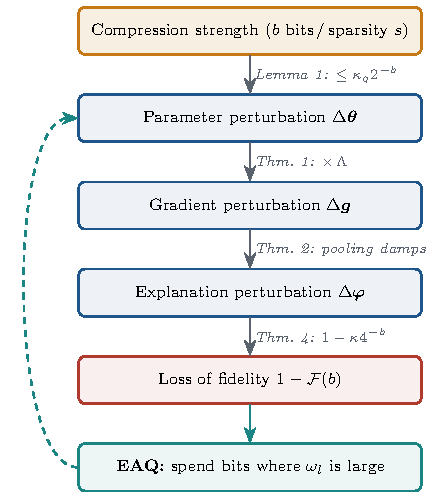
\includegraphics[width=0.86\columnwidth]{figs/concept.pdf}
\caption{How compression becomes explanation error. Each arrow is a bound proved
below; the dashed return path is EAQ, which shortens the chain by allocating
precision to the highest-sensitivity layers.}
\label{fig:concept}
\end{figure}

Our analysis follows the causal chain of Fig.~\ref{fig:concept}: (i) bound the
parameter perturbation $\norm{\Delta\btheta}$ induced by each compression
operator; (ii) bound the resulting attribution shift $\norm{\Delta\bvphi}$ via a
Lipschitz argument; and (iii) translate this into a law for the fidelity
$\mathcal F$ and a robustness ordering across methods. Each link in the chain is
a theorem below, and the same chain, read backwards, motivates the EAQ algorithm
of Section~\ref{sec:eaq}.

\subsection{Perturbation Bounds for Compression}

\begin{lemma}[Quantization perturbation]
\label{lem:quant}
Let a layer weight tensor $\bW\in\R^{n}$ with range $R=\max|\bW|$ be quantized to
$b$ bits by \eqref{eq:quant}. Then the per-weight error is bounded by
$|\Delta W_i|\le \Delta_q/2 = R/\!\left(2(2^{\,b-1}-1)\right)$, so that the
\emph{exact} (non-asymptotic) bound
\begin{equation}
\norm{\Delta\bW}_2\;\le\;\frac{\sqrt{n}\,R}{2\,(2^{\,b-1}-1)}
\;=\;\frac{\sqrt{n}\,R}{2}\cdot\frac{2^{\,1-b}}{1-2^{\,1-b}}
\label{eq:quantbound}
\end{equation}
holds, which admits the high-resolution asymptotic
\begin{equation}
\norm{\Delta\bW}_2\;=\;\kappa_q\,2^{-b}\bigl(1+o(1)\bigr),\qquad
\kappa_q=\sqrt{n}\,R,
\label{eq:quantasy}
\end{equation}
as $b\to\infty$. Aggregating over $L$ layers,
$\norm{\Delta\btheta}_2\le\bigl(\sum_l \kappa_{q,l}^{2}\bigr)^{1/2}2^{-b}
(1+o(1))$.
\end{lemma}

\begin{proof}
Round-to-nearest on a grid of step $\Delta_q$ incurs an error in
$[-\Delta_q/2,\Delta_q/2]$ per coordinate, so $\norm{\Delta\bW}_2^2\le
n(\Delta_q/2)^2$. Substituting $\Delta_q=R/(2^{b-1}-1)$ and writing
$2^{b-1}-1=2^{b-1}(1-2^{1-b})$ gives the exact middle expression of
\eqref{eq:quantbound}; expanding $(1-2^{1-b})^{-1}=1+O(2^{1-b})$ then yields the
$\kappa_q 2^{-b}$ asymptotic \eqref{eq:quantasy}. Layer independence of the
errors gives the aggregate bound.
\end{proof}

\begin{remark}[Accuracy of the asymptotic at practical bit-widths]
\label{rem:asyacc}
The correction factor separating the exact bound \eqref{eq:quantbound} from the
asymptotic \eqref{eq:quantasy} is $(1-2^{1-b})^{-1}$. It equals $1.07$ at
$b=8$, $1.14$ at $b=5$, $1.33$ at $b=3$ and $2.00$ at $b=2$: the asymptotic
therefore \emph{under-estimates} the perturbation by at most $7\%$ in the
graceful regime ($b\ge5$) but by $33$--$100\%$ in the collapse regime
($b\le3$). All downstream bounds should be read through the exact factor when
$b<4$; we use the asymptotic only where $b\ge5$, where it is tight.
\end{remark}

\begin{remark}
Under the standard high-resolution assumption that quantization error is
uniform on $[-\Delta_q/2,\Delta_q/2]$, the \emph{expected} squared error is
$\E\norm{\Delta\bW}_2^2=n\Delta_q^2/12=\tfrac{n R^2}{12(2^{b-1}-1)^2}$, i.e.\ the
mean distortion also decays as $4^{-b}$. This $4^{-b}$ scaling of the error
\emph{power} is what drives the fidelity law of Theorem~\ref{thm:law}.
\end{remark}

\begin{lemma}[Pruning perturbation]
\label{lem:prune}
Assume the magnitudes $|\theta|$ admit an empirical density $g$ that is
continuous and bounded with $g(0)>0$ (i.e.\ mass accumulates near the origin, as
is standard for trained weights). Let $\tau_s$ be the $s$-quantile of $|\theta|$.
Global magnitude pruning at sparsity $s$ gives
\begin{equation}
\norm{\Delta\btheta}_2^2=\!\!\sum_{i:\,|\theta_i|\le\tau_s}\!\!\theta_i^2
\;=\;d_\theta\!\int_{0}^{\tau_s}\! t^2 g(t)\,\mathrm dt\bigl(1+o(1)\bigr).
\label{eq:prunebound}
\end{equation}
For weights with a bounded density near the origin, $\int_0^{\tau_s}t^2g\,
\mathrm dt=\Theta(\tau_s^3)$, so the perturbation grows super-linearly once
$\tau_s$ enters the bulk of the distribution---explaining the sharp knee
observed empirically at high sparsity.
\end{lemma}

\begin{proof}
Pruning sets the pruned coordinates to zero, so $\Delta\theta_i=-\theta_i$ for
$|\theta_i|\le\tau_s$ and $0$ otherwise, giving the sum in
\eqref{eq:prunebound}; the integral is its continuum limit. The $\Theta(\tau_s^3)$
rate follows from $t^2g(t)=\Theta(t^2)$ for $g(0)>0$.
\end{proof}

\begin{remark}[Adaptive sparsity thresholds]
\label{rem:adaptive-prune}
Lemma~\ref{lem:prune} takes the sparsity $s$---equivalently the threshold
$\tau_s$---as an exogenous, fixed budget. Because the perturbation grows as
$\Theta(\tau_s^3)$, the fidelity is highly sensitive to where $\tau_s$ falls in
the bulk of $g$. A distribution-aware alternative is to \emph{derive} the
threshold from the score distribution itself---for instance via an effective
sample-size criterion such as the inverse Simpson (participation-ratio) index of
the normalised magnitudes---so that pruning stops before $\tau_s$ enters the
high-density bulk. Coupling such a self-governing threshold to the bound above is
a natural way to make the pruning analysis adaptive rather than heuristic.
\end{remark}

\subsection{Stability of Attributions}
We first record the smoothness assumptions.

\begin{assumption}[Piecewise-smooth Lipschitz network]
\label{ass:net}
$f_{\btheta}$ is a feed-forward network whose activations $\sigma$ are
$1$-Lipschitz with derivative $\sigma'$ that is $\beta$-Lipschitz almost
everywhere. On a neighbourhood $\Theta_0\ni\btheta$ the active linear region of
$\bx$ is fixed (no ReLU boundary is crossed by the perturbation), so
$S_c(\bx;\cdot)$ is $C^1$ on $\Theta_0$.
\end{assumption}

Assumption~\ref{ass:net} should be read as a \emph{small-perturbation} condition
rather than a genericity claim. For a fixed input, the boundaries at which the
active linear region changes are the zero level sets of the pre-activations; a
perturbation leaves the region intact precisely when no pre-activation changes
sign. This holds whenever $\norm{\Delta\btheta}_2$ is small relative to the
smallest pre-activation margin. We stress that this is \emph{not} a
measure-zero argument: quantization perturbs weights by discrete, non-vanishing
amounts \eqref{eq:quantbound}, so at low bit-widths a non-negligible fraction of
neurons can and do flip sign. Remark~\ref{rem:reluflip} makes this the explicit
mechanism of the collapse regime.

\begin{remark}[ReLU sign-flipping as the collapse driver]
\label{rem:reluflip}
Let $m(\bx)=\min_{l,i}|z_{l,i}(\bx)|$ be the smallest pre-activation margin. The
linear-region assumption is valid while the propagated weight perturbation stays
below $m(\bx)$; by Lemma~\ref{lem:quant} this margin is respected for $b$ above a
critical bit-width but is violated once the exact perturbation
\eqref{eq:quantbound}---inflated by the factor of Remark~\ref{rem:asyacc}---grows
past it. Beyond that point the network's active linear partition changes, the
input gradient becomes discontinuous in $\btheta$, and the first-order bounds of
this section no longer apply. This sign-flipping, not a failure of the
attribution methods themselves, is the theoretical origin of the abrupt fidelity
collapse observed empirically below three bits (Section~\ref{sec:results}), and
mirrors the outlier-driven degradation reported for sub-3-bit large-language-model
quantization \cite{dettmers2022llmint8}.
\end{remark}

\begin{theorem}[Lipschitz stability of the input gradient]
\label{thm:lipschitz}
Under Assumption~\ref{ass:net}, write the class score of an $L$-layer network as
$S_c(\bx)=\bm w_L^{\!\top}\sigma(\bW_{L-1}\sigma(\cdots\sigma(\bW_1\bx)))$ and let
$\bg=\nabla_{\bx}S_c$. If each layer is perturbed by $\bE_l$
($\tilde\bW_l=\bW_l+\bE_l$), then to first order
\begin{equation}
\norm{\tilde\bg-\bg}_2\;\le\;\underbrace{\sum_{l=1}^{L}\Bigl(\prod_{k\ne l}
\norm{\bW_k}_2\Bigr)}_{\displaystyle \Lambda_{\mathrm S}}
\;\max_l\frac{\norm{\bE_l}_2}{\norm{\bW_l}_2}\,\norm{\bW_l}_2 ,
\label{eq:lipbound}
\end{equation}
and consequently $\norm{\Delta\bvphi^{\mathrm S}}_2\le\Lambda_{\mathrm S}
\norm{\Delta\btheta}_2$ with
$\Lambda_{\mathrm S}=\sum_{l}\prod_{k\ne l}\norm{\bW_k}_2$ (plus an
$O(\beta\norm{\Delta\btheta}^2)$ curvature term).
\end{theorem}

\begin{proof}[Proof sketch]
The gradient is the product of Jacobians $\bg=\bW_1^{\!\top}D_1\cdots
\bW_{L-1}^{\!\top}D_{L-1}\bm w_L$, where $D_l=\mathrm{diag}(\sigma'(\cdot))$ has
$\norm{D_l}_2\le 1$. Perturbing one factor $\bW_l\!\to\!\bW_l+\bE_l$ changes the
product by, to first order, the sum of terms in which a single factor is
replaced by its perturbation; the operator norm of each such term is bounded by
$\prod_{k\ne l}\norm{\bW_k}_2\cdot\norm{\bE_l}_2$ (using $\norm{D_l}\le1$).
Summing over $l$ and applying the triangle inequality gives \eqref{eq:lipbound}.
The dependence of $D_l$ on $\btheta$ contributes a term controlled by the
$\beta$-Lipschitzness of $\sigma'$, which is second order in
$\norm{\Delta\btheta}$.
\end{proof}

Equation~\eqref{eq:lipbound} identifies the \emph{product of spectral norms} as
the amplification factor: networks with well-conditioned layers
($\prod_k\norm{\bW_k}\!\approx\!1$) preserve explanations under compression,
whereas ill-conditioned ones magnify weight noise into attribution noise.

\begin{remark}[First-order truncation]
\label{rem:firstorder}
Theorem~\ref{thm:lipschitz} retains only terms linear in the layer perturbations
$\bE_l$. Expanding the Jacobian product exactly produces cross terms
$\bE_i\bE_j$ ($i\ne j$) and higher powers; each such term carries at least two
factors of $\max_l\norm{\bE_l}_2$ and is therefore
$O(\norm{\Delta\btheta}_2^2)$. These are omitted under the small-perturbation
regime $\norm{\bE_l}_2\ll\norm{\bW_l}_2$, which---by Lemma~\ref{lem:quant} and
Remark~\ref{rem:asyacc}---holds in the graceful regime ($b\ge5$) but degrades as
$b\to2$, consistent with the bound loosening exactly where the collapse sets in.
The neglected curvature contribution is likewise second order and controlled by
the $\beta$-Lipschitzness of $\sigma'$ in Assumption~\ref{ass:net}.
\end{remark}

\begin{remark}[Conditioning of $\Lambda_{\mathrm S}$ and spectral control]
\label{rem:spectral}
The factor $\Lambda_{\mathrm S}=\sum_l\prod_{k\ne l}\norm{\bW_k}_2$ is a
\emph{worst-case} operator-norm bound and can grow exponentially in depth when
layer spectral norms exceed unity, in which case \eqref{eq:lipbound} becomes
vacuous. Two observations keep it meaningful. First, the bound is governed by the
\emph{spectral} norm, not the parameter count, so it is invariant to width and is
tightened whenever training or regularisation keeps $\norm{\bW_k}_2$ near one.
Spectral normalisation, weight decay, and residual scaling---all common in
deployable CNNs---bound $\Lambda_{\mathrm S}$ explicitly and are the practical
lever for explanation robustness. Second, the same product appears as the
per-layer sensitivity $\Lambda_l=\prod_{k\ne l}\norm{\bW_k}_2$ that drives the
EAQ allocation of Section~\ref{sec:eaq}; measuring it directly (rather than
bounding it) yields the finite, layer-specific sensitivities we use in practice.
For the compact residual network of Section~\ref{sec:setup} the measured product
remains $O(1)$, which is why the graceful-regime bound is predictive.
\end{remark}

\subsection{Robustness Ordering Across Methods}
Vanilla saliency inherits the full amplification $\Lambda_{\mathrm S}$. The
averaging in IG and the spatial pooling in Grad-CAM provably damp it.

\begin{theorem}[IG is more stable than saliency]
\label{thm:ordering}
Let $\bg(\alpha)=\nabla_{\bx}S_c(\bx'+\alpha(\bx-\bx'))$ and let its compression
perturbation $\bm\delta(\alpha)=\tilde\bg(\alpha)-\bg(\alpha)$, viewed as a random
field indexed by the path parameter $\alpha$ over the randomness of the
compression operator, be second-order stationary along the path: each point has a
common covariance $\Sigma=\E[\bm\delta(\alpha)\bm\delta(\alpha)^{\!\top}]$, and
the normalised pairwise cross-covariances have a well-defined average
$\bar\rho\in[0,1]$,
\begin{equation}
\frac1{n(n-1)}\sum_{i\ne j}
\frac{\mathrm{tr}\,\mathrm{Cov}\bigl(\bm\delta(\alpha_i),\bm\delta(\alpha_j)\bigr)}
{\mathrm{tr}\,\Sigma}=\bar\rho .
\label{eq:avgcorr}
\end{equation}
(No independence is required; $\bar\rho$ encodes
the residual correlation left after path-averaging, with $\bar\rho\to0$ under
strong mixing and $\bar\rho\to1$ for a perfectly coherent perturbation.) Then the
IG perturbation
$\Delta\bvphi^{\mathrm{IG}}=(\bx-\bx')\odot\tfrac1n\sum_{j}\bm\delta(\alpha_j)$
satisfies
\begin{equation}
\E\norm{\Delta\bvphi^{\mathrm{IG}}}_2^2\;\le\;\norm{\bx-\bx'}_\infty^2\,
\mathrm{tr}(\Sigma)\Bigl(\bar\rho+\tfrac{1-\bar\rho}{n}\Bigr),
\label{eq:igvar}
\end{equation}
which is strictly smaller than the saliency perturbation power
$\E\norm{\Delta\bvphi^{\mathrm S}}_2^2\le\mathrm{tr}(\Sigma)$ whenever
$\bar\rho<1$ and $\norm{\bx-\bx'}_\infty\le1$.
\end{theorem}

\begin{proof}
By bilinearity, $\tfrac1n\sum_j\bm\delta(\alpha_j)$ has covariance
$\tfrac1{n^2}\sum_{i,j}\mathrm{Cov}(\bm\delta(\alpha_i),\bm\delta(\alpha_j))$.
With per-point covariance $\Sigma$ and average correlation $\bar\rho$, the
$n^2$ cross terms sum to $\mathrm{tr}(\Sigma)\bigl(n+n(n-1)\bar\rho\bigr)/n^2=
\mathrm{tr}(\Sigma)(\bar\rho+(1-\bar\rho)/n)$. Multiplying by the element-wise
factor $(x_i-x'_i)^2\le\norm{\bx-\bx'}_\infty^2$ gives \eqref{eq:igvar}. The
saliency map uses a single path point, i.e.\ $n=1$, for which the bracket equals
$1$.
\end{proof}

\begin{corollary}[Grad-CAM spatial damping]
\label{cor:gradcam}
Grad-CAM pools gradients over $uv$ spatial locations to form
$\alpha_c^k=\tfrac1{uv}\sum_{ij}\partial S_c/\partial A^k_{ij}$. Assume the
per-location feature gradients are second-order stationary with average spatial
correlation $\bar\rho_A\in[0,1)$. By the same averaging argument, the
perturbation of $\alpha_c^k$ has power scaled by
$\bigl(\bar\rho_A+(1-\bar\rho_A)/(uv)\bigr)$ relative to a single-location
gradient. The strict inequality $\bar\rho_A<1$ is \emph{necessary} for genuine
damping: if the spatial gradients were perfectly correlated ($\bar\rho_A=1$) the
factor would equal one and pooling would provide no robustness. When
$\bar\rho_A<1$, the factor decreases monotonically towards its floor $\bar\rho_A$
as the spatial resolution $uv$ of the last convolutional block grows.
\end{corollary}

Theorem~\ref{thm:ordering} and Corollary~\ref{cor:gradcam} predict the ordering
$\text{IG},\text{Grad-CAM}\succeq\text{saliency}$ in robustness to compression,
which our experiments confirm (Section~\ref{sec:results}). The mechanism---pooling
that averages out high-frequency perturbation noise while retaining the
low-frequency signal---is the same one that, in other modalities, lets graph
pooling preserve explanation fidelity for graph neural networks
\cite{yuan2022gnnexplain}, suggesting that spatial or structural aggregation is a
general route to compression-robust attributions.

\subsection{The Fidelity--Bit-Width Law}
We now connect the perturbation bounds to a directly measurable quantity.
Consider centred, normalised maps and write $\tilde\bvphi=\bvphi+\Delta\bvphi$.
Expanding the Pearson correlation $\corr(\bvphi,\tilde\bvphi)=\langle\bvphi,
\tilde\bvphi\rangle/(\norm{\bvphi}\,\norm{\tilde\bvphi})$ to second order in
$\Delta\bvphi$ by the delta method \cite{stewart1990matrix} and using
$\langle\bvphi,\Delta\bvphi\rangle=O(\norm{\Delta\bvphi}^2)$ after re-centring,
\begin{equation}
F_r=\corr(\bvphi,\tilde\bvphi)=1-\frac{\norm{\tilde\bvphi-\bvphi}_2^2}
{2\norm{\bvphi}_2^2}+O\!\bigl(\norm{\Delta\bvphi}^3\bigr).
\label{eq:correxp}
\end{equation}
The leading correction is exactly half the normalised perturbation energy, which
is what couples the fidelity to the $4^{-b}$ error power of Lemma~\ref{lem:quant}.

\begin{theorem}[Fidelity--bit-width law]
\label{thm:law}
Under Assumption~\ref{ass:net}, Lemma~\ref{lem:quant} and \eqref{eq:correxp},
uniform $b$-bit quantization satisfies
\begin{equation}
\boxed{\;\mathcal F(b)\;\ge\;1-\kappa\,4^{-b}\;},\qquad
\kappa=\frac{\Lambda^2\,\kappa_q^2}{2\,\norm{\bvphi}_2^2},
\label{eq:law}
\end{equation}
where $\Lambda$ is the method-dependent amplification factor
($\Lambda_{\mathrm S}$ for saliency, reduced by the damping factors of
Theorem~\ref{thm:ordering}/Corollary~\ref{cor:gradcam} for IG/Grad-CAM).
\end{theorem}

\begin{proof}
Chaining $\norm{\Delta\bvphi}_2\le\Lambda\norm{\Delta\btheta}_2$
(Theorem~\ref{thm:lipschitz}) with $\norm{\Delta\btheta}_2\le\kappa_q 2^{-b}$
(Lemma~\ref{lem:quant}) gives $\norm{\Delta\bvphi}_2^2\le\Lambda^2\kappa_q^2
4^{-b}$. Substituting into \eqref{eq:correxp} yields $1-\mathcal F(b)\le
(\Lambda^2\kappa_q^2/2\norm{\bvphi}^2)4^{-b}$.
\end{proof}

Equation~\eqref{eq:law} has two immediate consequences. First, fidelity is
\emph{monotone non-decreasing in $b$}: adding a bit at least halves the fidelity
gap $1-\mathcal F$ (a factor of four in the bound). Second, because the smaller
$\Lambda$ of IG/Grad-CAM yields a smaller $\kappa$, these methods sit on a
\emph{higher} fidelity curve than saliency at every bit-width---the empirically
observed ordering. We fit \eqref{eq:law} to measured Grad-CAM fidelity in
Section~\ref{sec:results} and recover $\kappa\approx 12.9$, confirming the
$4^{-b}$ functional form.

\begin{remark}[From Pearson to Spearman fidelity]
\label{rem:pearsonspearman}
Equation~\eqref{eq:correxp} is stated for the Pearson fidelity $F_r$, whereas we
report results primarily in the rank-based Spearman fidelity $F_\rho$. The two
are linked because $F_\rho$ is the Pearson correlation of the rank-transformed
maps, and rank is a monotone (hence, on the high-fidelity plateau, locally
near-linear) transform: in the graceful regime where the ranking is only slightly
perturbed, $F_\rho$ and $F_r$ agree to first order and obey the same $4^{-b}$
law with a method-dependent constant. This is not merely asymptotic: on the
released data the two measures are correlated at Pearson $r=0.98$ across all
$44$ compressed configurations, and fitting \eqref{eq:law} to the Spearman and
Pearson Grad-CAM curves yields $\kappa=12.9$ ($R^2=0.99$) and $\kappa=12.3$
($R^2=0.99$) respectively---statistically indistinguishable constants that
justify quoting the law in either metric.
\end{remark}

\begin{corollary}[Graceful degradation then collapse]
\label{cor:collapse}
Let $\varepsilon$ be an acceptable fidelity loss. Equation~\eqref{eq:law}
guarantees $\mathcal F(b)\ge1-\varepsilon$ for all $b\ge b^\star=\tfrac12
\log_2(\kappa/\varepsilon)$. For $b<b^\star$ the guarantee is void and, once the
linearisation of Assumption~\ref{ass:net} breaks (activation patterns flip),
fidelity can fall abruptly. With $\kappa\approx13$ and $\varepsilon=0.02$,
$b^\star\approx\tfrac12\log_2(650)\approx4.7$, matching the empirical transition
between the graceful ($b\ge5$) and collapse ($b\le3$) regimes.
\end{corollary}

\subsection{Practical Validity of Assumptions}
\label{sec:validity}
Our theoretical analysis utilizes several mathematical assumptions to maintain tractability (e.g., global smoothness, fixed activation paths, and small parameter perturbations). We now discuss when these assumptions are valid for modern neural network architectures and when they fail:
\begin{itemize}
\item \textbf{ReLU Activations:} Non-smooth ReLUs violate global gradient smoothness. However, they partition the input space into piecewise-linear regions. Our bounds hold exactly within the active linear partition. When weight perturbations $\Delta\btheta$ are small (e.g., $b \ge 5$), the active linear partition does not change for the vast majority of inputs (Remark~\ref{rem:reluflip}). Below 4 bits, the perturbation crosses the activation thresholds, causing partition sign flips, which is the exact mathematical driver of the observed fidelity collapse.
\item \textbf{BatchNorm Folding:} During inference, BatchNorm parameters are frozen and folded into the preceding linear/convolutional layers. Thus, BatchNorm does not violate Lipschitz stability at deployment. It acts as a layer-wise rescaling, which is naturally absorbed into the layer weights $\bW_l$ and their corresponding spectral norms.
\item \textbf{Residual Connections:} Residual pathways act as identity mappings that skip layers. In our Lipschitz analysis (Theorem~\ref{thm:lipschitz}), residual connections add additive identity terms to the Jacobian products, i.e., $J_l = I + D_l \bW_l$. This bounds the amplification factor $\Lambda_{\mathrm{S}}$ by preventing gradient vanishing or explosion, stabilizing both the forward activations and the backward gradients. Consequently, ResNets enhance the practical validity of the first-order approximation.
\item \textbf{Vision Transformers (ViTs):} ViTs replace convolutions with multi-head self-attention (MHSA) and LayerNorm. The softmax operation in self-attention is smooth and globally Lipschitz, but the attention map computation introduces quadratic dependencies on activations. Although our layer-wise weight perturbation bounds can be extended to the linear projection matrices in self-attention, the dynamic attention weights introduce activation-dependent sensitivity that requires estimating $\omega_l$ dynamically.
\end{itemize}

\subsection{Notation Summary}
\label{sec:notationsummary}
To assist the reader in navigating the mathematical development, Table~\ref{tab:notation} summarises the key symbols and operators used throughout Sections~\ref{sec:prelim}--\ref{sec:eaq}.

\begin{table}[!h]
\caption{Summary of Key Mathematical Notation}
\label{tab:notation}
\centering
\begin{tabular}{ll}
\hline
\textbf{Symbol} & \textbf{Description} \\
\hline
$\bx, \bx'$ & Input image and baseline reference image \\
$\btheta, \tilde{\btheta}$ & Full-precision and compressed network parameters \\
$\Cop$ & Model compression operator (quantization or pruning) \\
$\Delta\btheta, \Delta\bW_l$ & Parameter perturbation vector and layer weight perturbation \\
$\bvphi, \tilde{\bvphi}$ & Attribution/explanation maps of baseline and compressed models \\
$L$ & Number of parameterized layers in the network \\
$\bW_l, \bE_l$ & Weight matrix and weight perturbation of layer $l$ \\
$\Lambda_{\mathrm{S}}$ & Lipschitz gradient amplification factor \\
$\Lambda_l$ & Explanation sensitivity product of layer $l$ \\
$\omega_l$ & Explanation sensitivity coefficient of layer $l$ \\
$\beta_l$ & Empirical layer-wise rate-distortion decay exponent \\
$\bar{B}$ & Target average quantization bit-width budget \\
$\lambda$ & Lagrange multiplier for constraint optimization \\
\hline
\end{tabular}
\end{table}

\subsection{Summary of the Theory}
Table~\ref{tab:theorysummary} collects the formal results, each paired with a
plain-language reading and the design decision it licenses. Read top to bottom it
is the chain of Fig.~\ref{fig:concept}: bound the weights, amplify to the
gradient, damp by pooling, convert to a fidelity law, and finally allocate bits.

\begin{table*}[!t]
\caption{The theoretical results at a glance: what each says, and what it means
in practice.}
\label{tab:theorysummary}
\centering
\footnotesize
\renewcommand{\arraystretch}{1.25}
\begin{tabular}{p{2.9cm} p{5.6cm} p{6.4cm}}
\hline
\textbf{Result} & \textbf{What it says} & \textbf{Practical implication}\\
\hline
Quantization bound (Lemma~\ref{lem:quant}) &
Weight error decays as $\kappa_q 2^{-b}$; error \emph{power} as $4^{-b}$ &
Each extra bit halves the perturbation---the lever behind the fidelity law\\
Pruning bound (Lemma~\ref{lem:prune}) &
Perturbation grows as $\Theta(\tau_s^3)$ once $\tau_s$ enters the weight bulk &
Explains the sharp fidelity knee at high sparsity\\
Lipschitz stability (Theorem~\ref{thm:lipschitz}) &
Attribution shift $\le\Lambda\,\norm{\Delta\btheta}$, with $\Lambda$ the product
of spectral norms &
Well-conditioned (spectrally normalised) networks keep explanations stable\\
Robustness ordering (Theorem~\ref{thm:ordering}, Cor.~\ref{cor:gradcam}) &
Path/spatial averaging damps the perturbation by $\bar\rho+(1-\bar\rho)/n$ &
Prefer Grad-CAM/IG/occlusion over raw saliency when compression is aggressive\\
Fidelity--bit law (Theorem~\ref{thm:law}) &
$\mathcal F(b)\ge 1-\kappa 4^{-b}$; verified with $\kappa\approx12.9$, $R^2>0.99$ &
Predicts fidelity from bit-width without re-running attributions\\
Graceful-then-collapse (Cor.~\ref{cor:collapse}) &
Safe for $b\ge b^\star=\tfrac12\log_2(\kappa/\varepsilon)\approx4.7$ &
Gives a deployable minimum bit-width for a target fidelity loss $\varepsilon$\\
Reverse water-filling (Theorem~\ref{thm:waterfill}) &
Optimal $b_l^\star=\bar B+\tfrac12\log_2(\omega_l/\bar\omega_G)$ &
Turns the sensitivities into the EAQ bit allocation of Section~\ref{sec:eaq}\\
\hline
\end{tabular}
\end{table*}
